% =====================================================================
%  Draft manuscript -- UAV swarm formation control with a modified APF
%  Status (2026-10-10): method + analysis + evaluation protocol written.
%  Simulation results and conclusions are NOT yet available; the places
%  where they will go are marked with  %% TODO(results)  in this source.
%  Compile:  latexmk -pdf main.tex
% =====================================================================
\documentclass[11pt]{article}

\usepackage[a4paper,margin=2.5cm]{geometry}
\usepackage[T1]{fontenc}
\usepackage[utf8]{inputenc}
\IfFileExists{lmodern.sty}{\usepackage{lmodern}}{}
\usepackage[protrusion=true,expansion=false]{microtype}
\usepackage{amsmath,amssymb,amsthm,mathtools,bm}
\usepackage{booktabs,threeparttable,array}
\usepackage{siunitx}
\usepackage{enumitem}
\usepackage{graphicx}
\usepackage{xcolor}
\usepackage{tikz}
\usetikzlibrary{arrows.meta,calc,decorations.pathreplacing}
\usepackage[ruled,vlined,linesnumbered]{algorithm2e}
\usepackage[numbers,sort&compress]{natbib}
\usepackage[colorlinks=true,linkcolor=blue!50!black,citecolor=blue!50!black,urlcolor=blue!50!black]{hyperref}
\usepackage[capitalise,nameinlink]{cleveref}

% ---------- theorem environments ----------
\newtheorem{assumption}{Assumption}
\newtheorem{lemma}{Lemma}
\newtheorem{theorem}{Theorem}
\newtheorem{proposition}{Proposition}
\newtheorem{corollary}{Corollary}
\theoremstyle{definition}
\newtheorem{definition}{Definition}
\theoremstyle{remark}
\newtheorem{remark}{Remark}
\crefname{assumption}{Assumption}{Assumptions}

% ---------- notation ----------
\newcommand{\R}{\mathbb{R}}
\newcommand{\bp}{\mathbf{p}}
\newcommand{\bv}{\mathbf{v}}
\newcommand{\bu}{\mathbf{u}}
\newcommand{\bx}{\mathbf{x}}
\newcommand{\ba}{\mathbf{a}}
\newcommand{\bI}{\mathbf{I}}
\newcommand{\bS}{\mathbf{S}}
\newcommand{\bD}{\mathbf{D}}
\newcommand{\bG}{\mathbf{G}}
\newcommand{\bQ}{\mathbf{Q}}
\newcommand{\bL}{\mathbf{L}}
\newcommand{\bdelta}{\bm{\delta}}
\newcommand{\bomega}{\bm{\omega}}
\newcommand{\bn}{\hat{\mathbf{n}}}
\newcommand{\bt}{\hat{\mathbf{t}}}
\newcommand{\norm}[1]{\left\lVert #1 \right\rVert}
\newcommand{\pos}[1]{\left[#1\right]_{+}}
\newcommand{\dmin}{d_{\min}}
\newcommand{\amax}{a_{\max}}
\newcommand{\Free}{\mathcal{F}}
\newcommand{\todo}[1]{\textcolor{red!70!black}{[TODO: #1]}}

\title{\textbf{Provably Safe and Smooth Formation Control of UAV Swarms\\
via a Modified Artificial Potential Field with Gyroscopic Escape\\
and PSD-Projected Potential-Rate Damping}\\[0.4em]
\large Working draft --- method, analysis and evaluation protocol}

\author{Tuan\thanks{\todo{full name, affiliation, e-mail; co-authors and supervisor}}}
\date{Draft of 10 October 2026}

\begin{document}
\maketitle

% =====================================================================
\begin{abstract}
Artificial potential fields (APFs) remain attractive for real-time control of
unmanned aerial vehicle (UAV) swarms because they are optimization-free,
distributed and naturally suited to energy-based stability analysis. Their
practical use, however, is limited by four coupled deficiencies: goals that are
non-reachable when obstacles are nearby (GNRON), spurious local minima,
oscillations and acceleration surges, and the lack of a guaranteed minimum
separation between agents in cluttered space. This paper proposes a distributed
second-order APF controller that addresses the four issues inside a single
energy function. The controller combines (i) a goal-normalized obstacle
repulsion that makes every formation slot an equilibrium; (ii) a Morse-type
formation coupling augmented with a barrier term that diverges at the minimum
separation; (iii) a gyroscopic escape force of the form $\bomega\times\bv$,
which bends trajectories around obstacles while doing zero mechanical work,
complemented by a stall-triggered hybrid reset; and (iv) a potential-rate
damping term assembled from positive-semidefinite projections of local Hessians,
which stays dissipative where the potential is non-convex and is available in
closed form from local measurements. Using the total mechanical energy as a
Lyapunov function, we prove that the closed loop keeps an explicit positive
margin above the minimum inter-agent distance, never reaches an obstacle,
remains bounded, and converges to the critical set of the potential; every
trajectory whose initial energy lies below the lowest spurious critical level
converges to the desired formation, and bounded hybrid resets preserve the
safety guarantee. A two-layer evaluation protocol---Monte Carlo point-mass
simulation and PX4 software-in-the-loop flight in ROS~2/Gazebo, with five
baselines and component ablations---is specified. The simulation study is in
progress and is not reported in this draft.
\end{abstract}

\noindent\textbf{Keywords:} UAV swarm; formation control; artificial potential
field; collision avoidance; local minima; Lyapunov stability; gyroscopic force;
potential-rate damping.

% =====================================================================
\section{Introduction}\label{sec:intro}

Missions such as search and rescue, infrastructure inspection, environmental
monitoring and urban logistics increasingly rely on teams of UAVs rather than a
single vehicle, because a swarm enlarges coverage, tolerates individual
failures and shortens mission time~\cite{chung2018survey,zhou2022swarm}. Flying
many vehicles close together, however, creates a two-fold safety problem: each
UAV must avoid static and moving obstacles \emph{and} its own teammates, while
the swarm should keep a prescribed geometric formation so that sensing and
communication remain coordinated. The controller that solves this problem must
run on embedded hardware at a high rate, typically above \SI{100}{\hertz} on a
flight controller or a low-cost companion computer.

Existing approaches fall into several families. Graph- and sampling-based
planners (A$^\ast$, RRT$^\ast$) find global paths but must re-plan continuously
in dynamic scenes and scale poorly when the joint configuration space of many
agents is searched. Model predictive control (MPC) handles constraints
explicitly but solves an optimization problem at every step. Multi-agent
reinforcement learning (MARL) adapts to complex environments but is expensive to
train and offers few guarantees outside its training distribution. Control
barrier functions (CBFs) provide rigorous safety guarantees~\cite{wang2017barrier}
but act as a safety filter that still requires a nominal formation controller
and a quadratic program at every step. Artificial potential fields
(APFs)~\cite{khatib1986} occupy a distinct niche: the control action is an
analytic gradient, the cost per agent is linear in the number of neighbours and
nearby obstacles, and the potential doubles as an energy function for stability
analysis. APFs remain in active use, often as the safety or guidance layer
underneath learning-based planners~\cite{zhao2026stamaddpg,shibu2026skysim}.

Four well-known deficiencies limit APF-based swarm control:
\begin{enumerate}[label=(D\arabic*),leftmargin=*]
  \item \textbf{GNRON.} When a goal lies inside the influence region of an
    obstacle, repulsion outweighs attraction at the goal, so the agent cannot
    settle there~\cite{ge2000}. In formation control every formation slot is a
    goal, so the problem appears whenever the formation passes close to an
    obstacle.
  \item \textbf{Local minima.} Attractive and repulsive forces can cancel at
    points other than the goal, trapping agents in front of obstacles or in
    concave regions~\cite{koren1991}.
  \item \textbf{Oscillations and acceleration surges.} Rapid changes of the
    gradient, particularly when the current and desired formations conflict,
    produce oscillatory paths and acceleration spikes that saturate the
    actuators~\cite{han2025time}.
  \item \textbf{Inter-agent separation.} Physics-inspired pair potentials such
    as Lennard-Jones and Morse produce a natural equilibrium spacing~\cite{xu2025consensus},
    but on their own they do not certify a minimum separation when the swarm
    is squeezed by obstacles.
\end{enumerate}
Each deficiency has been addressed in isolation. Rotational or vortex fields
remove local minima~\cite{hou2026irapf,manteaux2024rapf}, but position-dependent
rotational forces are non-conservative and invalidate the energy argument that
makes APFs attractive in the first place. Damping derived from the time
derivative of APF gradients suppresses oscillations~\cite{li2024lowosc,han2025time};
a direct implementation of the rate $\tfrac{d}{dt}\nabla U = \nabla^2 U\,\dot{\bp}$,
however, contains the Hessian of the potential, whose tangential curvature is
negative around every decreasing radial repulsion, so the term can inject
energy precisely when agents skirt obstacles or each other. To our knowledge no
existing controller treats the four deficiencies jointly under a single
Lyapunov function.

\paragraph{Contributions.} This paper makes the following contributions.
\begin{enumerate}[label=(C\arabic*),leftmargin=*]
  \item A \emph{unified swarm potential} combining a formation attraction, a
    goal-normalized obstacle repulsion in the spirit of~\cite{ge2000}, and a
    Morse formation coupling with a separation barrier. The desired formation is
    the unique global minimizer of the potential, and the potential diverges on
    the boundary of the collision-free set (\cref{sec:method,lem:potential}).
  \item A \emph{gyroscopic escape force} $\bomega_i(\bp_i)\times\bv_i$ whose
    rotation axis is chosen so that the deflection points towards the goal side
    of the nearest obstacle. Because the force is always orthogonal to the
    velocity it does no work, so it can be added without modifying the energy
    argument. A stall-triggered hybrid reset handles the case of zero velocity.
  \item A \emph{PSD-projected potential-rate damping} term that refines the
    time-derivative damping idea of~\cite{li2024lowosc,han2025time}: each local
    Hessian is projected onto the positive-semidefinite cone before use, which
    keeps the term dissipative everywhere, coincides with $\tfrac{d}{dt}\nabla U$
    wherever the local potentials are convex, and admits a closed form for
    radial pair potentials (\cref{lem:psd}).
  \item A \emph{Lyapunov analysis} establishing an explicit inter-agent
    separation margin, obstacle avoidance, boundedness, convergence to the
    critical set, convergence to the desired formation from every initial
    energy below the lowest spurious critical level, and robustness of these
    guarantees to bounded hybrid resets and to input saturation on the reached
    sublevel set (\cref{sec:analysis}).
  \item A \emph{reproducible evaluation protocol}: six scenarios, five
    baselines, seven metrics, component ablations and a two-layer simulation
    pipeline from point masses to PX4 software-in-the-loop (\cref{sec:protocol}).
\end{enumerate}

\paragraph{Organization.} \Cref{sec:related} reviews related work.
\Cref{sec:problem} states the problem. \Cref{sec:method} presents the
controller and \cref{sec:analysis} analyses it. \Cref{sec:protocol} specifies
the evaluation protocol, and \cref{sec:limitations} discusses limitations and
ongoing work.
%% TODO(results): add "Section X reports simulation results" once available.

% =====================================================================
\section{Related Work}\label{sec:related}

\subsection{Classical potential fields and the GNRON problem}
Khatib~\cite{khatib1986} introduced real-time obstacle avoidance with an
attractive quadratic potential towards the goal and a repulsive potential
$\tfrac12\eta(1/\rho-1/\rho_0)^2$ active within a distance $\rho_0$ of each
obstacle. Koren and Borenstein~\cite{koren1991} catalogued the inherent
limitations of this construction: trap situations due to local minima, no
passage between closely spaced obstacles, and oscillations in narrow passages
and in the presence of obstacles. Ge and Cui~\cite{ge2000} identified the GNRON
problem and multiplied the repulsive potential by a power of the distance to the
goal, so that repulsion vanishes at the goal and the goal becomes the global
minimum. Our obstacle term (\cref{sec:repulsion}) applies the same idea to
formation slots.

\subsection{Flocking and physics-inspired pair potentials}
Olfati-Saber~\cite{olfati2006} established a rigorous theory of flocking for
second-order agents, combining a gradient term from a bounded pairwise action
function, a velocity-consensus term, obstacle avoidance through virtual
$\beta$-agents, and navigational feedback. The total energy (relative kinetic
plus pairwise potential) serves as a Lyapunov function, and the closed loop
converges to $\alpha$-lattices without collisions under suitable conditions.
More recently, Xu~et~al.~\cite{xu2025consensus} modelled a UAV swarm as a
molecular system on top of the Vicsek framework, using the
Lennard-Jones~\cite{lennardjones1924} and Morse~\cite{morse1929} potentials for
attraction and repulsion, a velocity-consensus term and pinning control from a
virtual leader. They proved stability with an energy function and reported that
the Morse potential yields better consensus than Lennard-Jones. Neither work
prescribes an arbitrary geometric formation, and the Morse potential is bounded
at short range, which motivates the barrier term in our design.

\subsection{Escaping local minima}
A common remedy is to add a force tangential to the obstacle. Hou~et~al.~\cite{hou2026irapf}
replaced Euclidean repulsion with a superellipse-norm potential that conforms to
obstacle shapes and introduced a dynamically selected rotational force whose
tangential direction aligns with the goal vector; the APF parameters are tuned
by multi-agent proximal policy optimization. Kim~et~al.~\cite{kim2024wallfollower}
switch to a wall-following mode that incrementally rotates the attractive force
when the total force becomes small, then return to the APF. Ma~et~al.~\cite{ma2025sa}
initialise an escape force from the repulsion at the time of entrapment and
rotate it with a direction rule based on the side of the repulsive force
relative to the attractive one. Rotated vector fields, as reviewed and extended in~\cite{manteaux2024rapf},
turn the repulsive field around each obstacle into a vortex of the same
magnitude within the influence radius. All these forces depend on position, so
they generally do work along trajectories and the energy-based stability
argument no longer applies. Our escape force depends on velocity and is
orthogonal to it, which preserves the argument.

\subsection{Suppressing oscillations and acceleration surges}
Li~et~al.~\cite{li2024lowosc} generated collision damping terms by
differentiating the APF gradient with respect to time and proved stability with
an energy-based Lyapunov function. Han~et~al.~\cite{han2025time} developed this
idea into a unified framework for attractive and repulsive APFs in
time-variant formation tracking, in which the gradients transfer energy between
potential and kinetic forms and the time derivatives of the gradients act as
damping; they proved Lyapunov stability and collision avoidance and analysed
manoeuvrability geometrically. We adopt their potential-rate damping principle
and modify it so that it is dissipative by construction (\cref{sec:damping}).
Zhang~et~al.~\cite{zhang2026closedform} proposed a closed-form distributed
formation controller with a virtual centroid, a generalized $p$-norm collision
measure, an event-triggered avoidance vector activated only when the collision
risk increases, and a deadlock perturbation; in their simulations the method
achieved smaller avoidance peaks and smoother speed and heading profiles than a
traditional APF. Bui~et~al.~\cite{bui2025event} navigated robot swarms through
narrow spaces with APF-designed behaviours (goal seeking, formation
maintenance, tailgating, collision avoidance) and event-based reconfiguration,
with Lyapunov-based formation stability.

\subsection{Optimization- and learning-based approaches}
Safety barrier certificates~\cite{wang2017barrier} and high-order CBFs~\cite{xiao2022hocbf}
minimally modify a nominal input through a quadratic program so that a safe set
is forward invariant. Optimal reciprocal collision avoidance (ORCA)~\cite{vandenberg2011orca}
selects, by linear programming, the velocity closest to a preferred one among
those that avoid every neighbour for a time horizon, with responsibility shared
between agents. Learning-based planners increasingly embed APFs: STA-MADDPG
uses a dynamic APF as state augmentation to accelerate convergence~\cite{zhao2026stamaddpg},
and SkySim filters language-model-generated waypoints through an APF safety
layer for Crazyflie swarms in ROS~2/Gazebo~\cite{shibu2026skysim}. A provably
safe APF is therefore useful both as a stand-alone controller and as a safety
layer for such systems.

\Cref{tab:related} summarises which deficiencies each line of work addresses,
as stated in the respective publications.

\begin{table}[htbp]
\centering
\begin{threeparttable}
\caption{Deficiencies addressed by representative approaches.}\label{tab:related}
\small
\begin{tabular}{@{}lcccccc@{}}
\toprule
Approach & D1 & D2 & D3 & D4 & Formal guarantee & Optimization-free \\
\midrule
Khatib APF~\cite{khatib1986}               & --          & --          & --          & $\circ$     & --          & \checkmark \\
Ge \& Cui~\cite{ge2000}                     & \checkmark  & --          & --          & --          & --          & \checkmark \\
Olfati-Saber~\cite{olfati2006}             & --          & --          & --          & \checkmark  & \checkmark  & \checkmark \\
Xu et al.~\cite{xu2025consensus}           & --          & --          & --          & \checkmark  & \checkmark  & \checkmark \\
Rotational APF~\cite{hou2026irapf,manteaux2024rapf} & --  & \checkmark  & --          & $\circ$     & --          & \checkmark \\
Potential-rate damping~\cite{han2025time}  & --          & --          & \checkmark  & \checkmark  & \checkmark  & \checkmark \\
Event-triggered closed form~\cite{zhang2026closedform} & -- & $\circ$  & \checkmark  & \checkmark  & \checkmark  & \checkmark \\
CBF-QP~\cite{wang2017barrier}              & --          & --          & --          & \checkmark  & \checkmark  & -- \\
\midrule
This work                                  & \checkmark  & \checkmark$^{\dagger}$ & \checkmark & \checkmark & \checkmark & \checkmark \\
\bottomrule
\end{tabular}
\begin{tablenotes}\footnotesize
\item[] D1: GNRON; D2: local minima; D3: smoothness (oscillations, acceleration
surges); D4: inter-agent separation.
\item[] \checkmark: addressed; $\circ$: partially addressed (e.g., collision
avoidance without a certified margin, or a deadlock perturbation without an
escape guarantee); --: not a stated objective.
\item[$\dagger$] Escape is promoted by the gyroscopic force and hybrid reset;
safety under escape is proved, while the escape rate is evaluated empirically.
\end{tablenotes}
\end{threeparttable}
\end{table}

% =====================================================================
\section{Problem Formulation}\label{sec:problem}

\subsection{Notation}
$\norm{\cdot}$ is the Euclidean norm, $\bI$ the $3\times3$ identity and
$[\bx]_\times$ the skew-symmetric matrix with $[\bx]_\times\mathbf{y}=\bx\times\mathbf{y}$.
For a symmetric matrix $\mathbf{M}=\sum_k\lambda_k\mathbf{e}_k\mathbf{e}_k^\top$,
$\pos{\mathbf{M}}=\sum_k\max(\lambda_k,0)\,\mathbf{e}_k\mathbf{e}_k^\top$ denotes
its projection onto the positive-semidefinite (PSD) cone, which is the nearest
PSD matrix in the Frobenius norm~\cite{higham1988}; for scalars
$[s]_+=\max(s,0)$. For $\bx\neq\mathbf{0}$, $\hat{\bx}=\operatorname{dir}(\bx)=\bx/\norm{\bx}$.

\subsection{Agent model}
The swarm has $N$ UAVs. As is common for multirotors flown with an inner
attitude and thrust loop (e.g., PX4~\cite{meier2015px4}), the outer loop of
UAV~$i$ is modelled as a double integrator with bounded acceleration:
\begin{equation}\label{eq:model}
  \dot{\bp}_i=\bv_i,\qquad \dot{\bv}_i=\mathrm{sat}_{\amax}(\bu_i),\qquad i=1,\dots,N,
\end{equation}
with position $\bp_i\in\R^3$, velocity $\bv_i\in\R^3$, commanded acceleration
$\bu_i\in\R^3$, and $\mathrm{sat}_{\amax}(\bu_i)
=\bu_i\min\{1,\amax/\norm{\bu_i}\}$ is norm saturation at $\amax>0$
(with $\mathrm{sat}_{\amax}(\mathbf{0})=\mathbf{0}$). The stacked vectors are
$\bp,\bv\in\R^{3N}$.

\subsection{Formation, obstacles and free space}
The desired formation is given by offsets $\bdelta_i$ about a formation centre
$\mathbf{c}$, so the slot of UAV~$i$ is $\bp_i^\star=\mathbf{c}+\bdelta_i$ and
the desired inter-agent distances are $d_{ij}^\star=\norm{\bdelta_i-\bdelta_j}$.
A set of formation edges $\mathcal{E}$ (an undirected graph) specifies which
pairs are coupled; $a_{ij}=1$ if $(i,j)\in\mathcal{E}$ and $0$ otherwise.

There are $M$ static obstacles $\mathcal{O}_k$, $k=1,\dots,M$, modelled as closed
balls with centres $\mathbf{o}_k$ and radii $R_k$ (vertical cylinders are
handled identically in the horizontal plane). The clearance of UAV~$i$ from
obstacle~$k$ and the outward unit normal are
\begin{equation}
  \rho_{ik}=\norm{\bp_i-\mathbf{o}_k}-R_k,\qquad \bn_{ik}=\nabla_{\bp_i}\rho_{ik}=\operatorname{dir}(\bp_i-\mathbf{o}_k).
\end{equation}
With $r_{ij}=\norm{\bp_i-\bp_j}$ and a minimum admissible separation $\dmin>0$,
the collision-free set is
\begin{equation}
  \Free=\bigl\{\bp\in\R^{3N}:\ \rho_{ik}>0\ \forall i,k;\ \ r_{ij}>\dmin\ \forall i\neq j\bigr\}.
\end{equation}

\subsection{Assumptions and objectives}
\begin{assumption}[Admissible formation]\label{as:formation}
Every slot lies outside every obstacle, $\rho_{ik}(\bp_i^\star)>0$, although it
may lie inside an obstacle's influence region. The barrier activation radius
$d_s$ satisfies $\dmin<d_s<\min_{i\neq j}d_{ij}^\star$.
\end{assumption}
\begin{assumption}[Information]\label{as:info}
UAV~$i$ knows its own state and slot, measures the relative position and
velocity of every UAV within a sensing radius $R_s\ge d_s$ and of its formation
neighbours $\{j:(i,j)\in\mathcal{E}\}$, and measures $\rho_{ik}$ and $\bn_{ik}$
for obstacles within a distance $\rho_0$.
\end{assumption}
\begin{assumption}[Regulation setting for the analysis]\label{as:static}
The obstacles and the formation centre $\mathbf{c}$ are stationary.
The extension to a moving centre is discussed in \cref{rem:tracking}.
\end{assumption}
\begin{assumption}[Initial condition]\label{as:init}
$\bp(0)\in\Free$.
\end{assumption}

\noindent The goal is to design $\bu_i$ from the information in \cref{as:info}
such that: (O1) $\bp(t)\in\Free$ for all $t\ge0$ with an explicit separation
margin; (O2) trajectories are bounded and converge to equilibria; (O3) the
desired formation $(\bp^\star,\mathbf{0})$ is asymptotically stable with an
explicit estimate of its region of attraction; (O4) the per-agent cost is
linear in the number of sensed neighbours and obstacles; and (O5) trajectories
are smooth, with few acceleration surges, which is assessed empirically in
\cref{sec:protocol}.

% =====================================================================
\section{Proposed Controller}\label{sec:method}

The controller is the negative gradient of a swarm potential $U$, plus linear
damping, PSD-projected potential-rate damping, and a gyroscopic escape force.
We describe the components in turn; \cref{alg:controller} summarises the
computation performed by each UAV.

\subsection{Formation attraction}
\begin{equation}\label{eq:Ua}
  U_a(\bp)=\sum_{i=1}^{N}\frac{k_a}{2}\norm{\bp_i-\bp_i^\star}^2,\qquad k_a>0.
\end{equation}

\subsection{Goal-normalized obstacle repulsion (component T1)}\label{sec:repulsion}
Let $g_i=\norm{\bp_i-\bp_i^\star}$ and, for an integer $m\ge3$,
\begin{equation}\label{eq:phi}
  \phi(\rho)=\begin{cases}\dfrac{\eta}{m}\left(\dfrac{1}{\rho}-\dfrac{1}{\rho_0}\right)^{m}, & 0<\rho\le\rho_0,\\[1ex] 0, & \rho>\rho_0.\end{cases}
\end{equation}
The obstacle potential is
\begin{equation}\label{eq:Ur}
  U_r(\bp)=\sum_{i=1}^{N}\sum_{k=1}^{M}\phi(\rho_{ik})\,g_i^{\,n},\qquad n\ge2 .
\end{equation}
Its gradient with respect to $\bp_i$ splits into a repulsive and a
goal-directed part, as in~\cite{ge2000}:
\begin{equation}\label{eq:Ur_grad}
  -\nabla_{\bp_i}U_r=\sum_{k}\Bigl[\underbrace{\frac{\eta}{\rho_{ik}^2}\Bigl(\frac{1}{\rho_{ik}}-\frac{1}{\rho_0}\Bigr)^{m-1}g_i^{\,n}\,\bn_{ik}}_{\text{away from obstacle}}\;\underbrace{-\,n\,\phi(\rho_{ik})\,g_i^{\,n-2}(\bp_i-\bp_i^\star)}_{\text{towards the slot}}\Bigr].
\end{equation}
Both parts vanish at $\bp_i=\bp_i^\star$ because $n\ge2$, so a slot inside an
obstacle's influence region remains an equilibrium. This removes the GNRON
problem. The exponent $m\ge3$ (instead of $m=2$ in~\cite{khatib1986,ge2000})
makes $\phi$ twice continuously differentiable with a locally Lipschitz second
derivative at $\rho_0$, which the damping term of \cref{sec:damping} requires.

\subsection{Morse formation coupling with separation barrier (component T2)}
For each pair $i\neq j$,
\begin{equation}\label{eq:psi}
  \psi_{ij}(r)=a_{ij}\,D_e\bigl(1-e^{-\alpha(r-d_{ij}^\star)}\bigr)^2+\psi_b(r),
\end{equation}
\begin{equation}\label{eq:barrier}
  \psi_b(r)=\begin{cases}\dfrac{k_b}{m}\left(\dfrac{1}{r-\dmin}-\dfrac{1}{d_s-\dmin}\right)^{m}, & \dmin<r\le d_s,\\[1ex] 0, & r>d_s,\end{cases}
\end{equation}
and $U_p(\bp)=\sum_{i<j}\psi_{ij}(r_{ij})$. The Morse term~\cite{morse1929,xu2025consensus}
couples formation neighbours elastically around their desired distance, which
keeps the relative geometry cohesive while individual UAVs deflect around
obstacles. Unlike the Lennard-Jones potential, it stays bounded at short range
and is numerically benign. The barrier term, active only below $d_s$ and
defined for every pair, diverges as $r\to\dmin^+$ and supplies the separation
guarantee that the Morse term lacks. By \cref{as:formation}, $\psi_b$ vanishes
in a neighbourhood of the desired formation.

The total potential is
\begin{equation}\label{eq:U}
  U(\bp)=U_a(\bp)+U_r(\bp)+U_p(\bp).
\end{equation}

\subsection{PSD-projected potential-rate damping (component T4)}\label{sec:damping}
Write $U=\sum_{e}U_e$ as a sum of local terms: one attraction term per agent,
one obstacle term $U_{ik}=\phi(\rho_{ik})g_i^n$ per agent-obstacle pair, and one
pair term $U_{ij}=\psi_{ij}(r_{ij})$ per agent pair. Each term depends on the
state of one or two agents only. For agent-obstacle terms let
$\bQ_{ik}=\nabla^2_{\bp_i}U_{ik}\in\R^{3\times3}$. For pair terms let
$\bx=\bp_i-\bp_j$, $r=\norm{\bx}$ and
\begin{equation}\label{eq:G}
  \bG_{ij}=\nabla^2_{\bx}\,\psi_{ij}(\norm{\bx})=\psi_{ij}''(r)\,\hat{\bx}\hat{\bx}^\top+\frac{\psi_{ij}'(r)}{r}\bigl(\bI-\hat{\bx}\hat{\bx}^\top\bigr).
\end{equation}
We define the damping matrix $\bD(\bp)\in\R^{3N\times3N}$ through its action on
$\bv$:
\begin{equation}\label{eq:Dv}
  [\bD(\bp)\bv]_i=k_a\bv_i+\sum_{k}\pos{\bQ_{ik}}\bv_i+\sum_{j\neq i}\pos{\bG_{ij}}(\bv_i-\bv_j).
\end{equation}
\Cref{lem:psd} shows that $\bD(\bp)$ is the sum of the PSD projections of the
Hessians of all local terms, so $\bD(\bp)\succeq0$. Three remarks motivate the
construction:
\begin{itemize}[leftmargin=*]
  \item If every local term is convex along the trajectory, then
    $\bD(\bp)\bv=\nabla^2U(\bp)\,\dot\bp=\tfrac{d}{dt}\nabla U(\bp(t))$, and
    $-K_r\bD\bv$ is exactly the potential-rate damping
    of~\cite{li2024lowosc,han2025time}. It opposes rapid changes of the
    potential force and thus suppresses acceleration surges.
  \item Around a decreasing radial repulsion ($\psi'<0$) the tangential
    curvature $\psi'/r$ in \eqref{eq:G} is negative, so $-K_r\bv^\top\nabla^2U\bv$
    can be positive when agents move tangentially around obstacles or
    neighbours. The projection removes these directions and keeps the term
    dissipative everywhere.
  \item For pair terms the projection has the closed form
    $\pos{\bG_{ij}}=[\psi_{ij}'']_+\hat\bx\hat\bx^\top+[\psi_{ij}'/r]_+(\bI-\hat\bx\hat\bx^\top)$,
    which uses only relative position and velocity. The $3\times3$ matrices
    $\pos{\bQ_{ik}}$ need one symmetric eigendecomposition each.
\end{itemize}

\subsection{Gyroscopic escape force (component T3)}
Let $\beta:\R_{>0}\to[0,1]$ be the $C^1$ activation $\beta(\rho)=\sigma\bigl((\rho_0-\rho)/(\rho_0-\rho_1)\bigr)$
with $0<\rho_1<\rho_0$ and $\sigma(s)=0$ for $s\le0$, $3s^2-2s^3$ for $0<s<1$
and $1$ for $s\ge1$. With gain $k_g\ge0$, bias $\mu>0$ and a common axis $\ba$
(we use the vertical unit vector $\mathbf{e}_z$), define
\begin{equation}\label{eq:omega}
  \bomega_i(\bp_i)=k_g\sum_{k}\beta(\rho_{ik})\Bigl[(\bp_i^\star-\bp_i)\times\bn_{ik}+\mu\,\ba\Bigr],
  \qquad \mathbf{f}^{\mathrm{gy}}_i=\bomega_i(\bp_i)\times\bv_i=[\bomega_i]_\times\bv_i .
\end{equation}
The force is orthogonal to $\bv_i$ and so does no work, as in the Lorentz force.
The axis is chosen so that the deflection points to the goal side of the
obstacle: if the UAV heads into the obstacle, $\bv_i=-s\,\bn_{ik}$ with $s>0$,
then with $\mathbf{g}=\bp_i^\star-\bp_i$ and $\ba$ ignored,
\begin{equation}
  (\mathbf{g}\times\bn_{ik})\times(-s\,\bn_{ik})=s\bigl(\mathbf{g}-(\mathbf{g}^\top\bn_{ik})\bn_{ik}\bigr),
\end{equation}
which is the component of the goal direction tangent to the obstacle. In the
symmetric trap ($\mathbf{g}\parallel\bn_{ik}$) the cross product vanishes and the
bias $\mu\ba$ breaks the symmetry with the same sense of rotation for all UAVs.
This acts like a shared traffic rule and avoids reciprocal dances between
agents that circumvent the same obstacle. The unnormalised factor
$(\bp_i^\star-\bp_i)$ keeps $\bomega_i$ locally Lipschitz and makes the
goal-directed rotation fade near the slot.

\Cref{fig:gyro} illustrates the mechanism.

\begin{figure}[htbp]
\centering
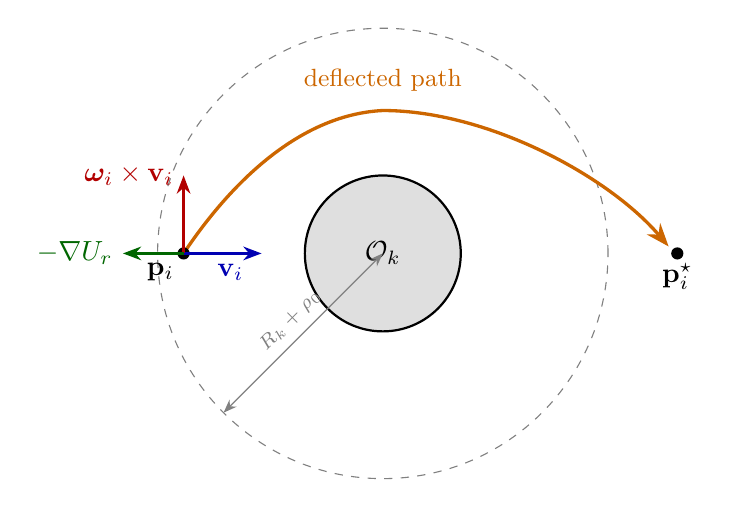
\begin{tikzpicture}[scale=1.1,>=Stealth]
  \fill[gray!25] (0,0) circle (0.9);
  \draw[thick] (0,0) circle (0.9);
  \node at (0,0) {$\mathcal{O}_k$};
  \draw[dashed,gray] (0,0) circle (2.6);
  \draw[gray,<->] (0,0) -- node[above,sloped,font=\scriptsize]{$R_k+\rho_0$} (-1.838,-1.838);
  \fill (3.4,0) circle (2pt) node[below] {$\bp_i^\star$};
  \draw[very thick,orange!80!black,->] (-2.3,0) .. controls (-1.8,0.75) and (-1.0,1.6) .. (0,1.65)
     .. controls (1.2,1.65) and (2.6,0.9) .. (3.3,0.08);
  \node[orange!80!black,font=\small] at (0,2.0) {deflected path};
  \fill (-2.3,0) circle (2pt);
  \node[below left] at (-2.3,0) {$\bp_i$};
  \draw[->,thick,blue!70!black] (-2.3,0) -- (-1.4,0) node[below,pos=0.6] {$\bv_i$};
  \draw[->,thick,red!70!black] (-2.3,0) -- (-2.3,0.9) node[left] {$\bomega_i\times\bv_i$};
  \draw[->,thick,green!40!black] (-2.3,0) -- (-3.0,0) node[left] {$-\nabla U_r$};
\end{tikzpicture}
\caption{Symmetric trap: the slot lies directly behind the obstacle, so
attraction and repulsion are collinear and a pure APF stalls. The gyroscopic
force $\bomega_i\times\bv_i$ bends the velocity tangentially, and the bias axis
$\ba$ fixes the sense of rotation, without adding mechanical energy.}
\label{fig:gyro}
\end{figure}

\subsection{Control law}
The commanded acceleration of UAV~$i$ is
\begin{equation}\label{eq:control}
  \boxed{\;\bu_i=-\nabla_{\bp_i}U(\bp)-K_d\bv_i-K_r[\bD(\bp)\bv]_i+\bomega_i(\bp_i)\times\bv_i\;}
\end{equation}
with $K_d>0$ and $K_r\ge0$. By \cref{as:info}, every term is computable from
local measurements: the attraction from the own state, the obstacle terms from
sensed obstacles within $\rho_0$, the barrier terms from UAVs within $d_s\le R_s$,
and the Morse terms from formation neighbours. The cost per agent and per step
is $O(|\mathcal{N}_i|+|\mathcal{O}_i|)$, where $\mathcal{N}_i$ and
$\mathcal{O}_i$ are the sensed neighbours and obstacles.

\subsection{Stall-triggered hybrid reset}
At an equilibrium $\bv=\mathbf{0}$, so the gyroscopic force is zero and cannot by
itself release an agent that has already stopped. We therefore add a reset.
UAV~$i$ is \emph{stalled} if $\norm{\bv_i}\le\varepsilon_v$ and
$\norm{\bp_i-\bp_i^\star}\ge\varepsilon_p$ have held continuously for $T_s$
seconds, at least $\tau_d$ seconds have elapsed since its previous reset, and it
has been reset fewer than $K_{\max}$ times. A reset applies
\begin{equation}\label{eq:reset}
  \bv_i^+=\bv_i+\Delta\,\bt_i,\qquad
  \bt_i=\begin{cases}\operatorname{dir}\bigl(\bomega_i\times(-\bn_i^{\mathrm{c}})\bigr), & \text{if the argument is nonzero},\\
  \operatorname{dir}\bigl(\ba\times(\bp_i^\star-\bp_i)\bigr), & \text{otherwise},\end{cases}
\end{equation}
where $\bn_i^{\mathrm{c}}$ is the normal of the closest sensed obstacle and
$\Delta>0$. The reset direction coincides with the deflection the gyroscopic
force would produce for a unit velocity heading into the obstacle. On a real
vehicle the reset is implemented as a short velocity set-point step.

\begin{algorithm}[htbp]
\caption{Control step of UAV $i$ (period $\Delta t$)}\label{alg:controller}
\KwIn{own state $(\bp_i,\bv_i)$, slot $\bp_i^\star$; relative states of sensed UAVs $j$; $(\rho_{ik},\bn_{ik})$ of sensed obstacles}
\KwOut{acceleration set-point $\bu_i$}
$\mathbf{f}\gets -k_a(\bp_i-\bp_i^\star)$;\quad $\mathbf{d}\gets k_a\bv_i$;\quad $\bomega\gets\mathbf{0}$\;
\ForEach{sensed obstacle $k$ with $\rho_{ik}\le\rho_0$}{
  $\mathbf{f}\gets\mathbf{f}-\nabla_{\bp_i}U_{ik}$ \tcp*{Eq.~\eqref{eq:Ur_grad}}
  $\mathbf{d}\gets\mathbf{d}+\pos{\bQ_{ik}}\bv_i$ \tcp*{$3\times3$ eigendecomposition}
  $\bomega\gets\bomega+k_g\beta(\rho_{ik})[(\bp_i^\star-\bp_i)\times\bn_{ik}+\mu\ba]$\;
}
\ForEach{sensed UAV $j$ with $r_{ij}\le d_s$ or $(i,j)\in\mathcal{E}$}{
  $\bx\gets\bp_i-\bp_j$;\quad $\mathbf{f}\gets\mathbf{f}-\psi_{ij}'(\norm{\bx})\,\hat\bx$\;
  $\mathbf{d}\gets\mathbf{d}+\bigl([\psi_{ij}'']_+\hat\bx\hat\bx^\top+[\psi_{ij}'/\norm{\bx}]_+(\bI-\hat\bx\hat\bx^\top)\bigr)(\bv_i-\bv_j)$\;
}
$\bu_i\gets\mathbf{f}-K_d\bv_i-K_r\mathbf{d}+\bomega\times\bv_i$\;
\If{stall condition holds}{apply reset \eqref{eq:reset}}
\Return $\mathrm{sat}_{\amax}(\bu_i)$\;
\end{algorithm}

% =====================================================================
\section{Stability and Safety Analysis}\label{sec:analysis}

We analyse the closed loop \eqref{eq:model}, \eqref{eq:control} first without
saturation and resets, then add both. The candidate Lyapunov function is the
total mechanical energy
\begin{equation}\label{eq:V}
  V(\bp,\bv)=\frac12\norm{\bv}^2+U(\bp),
\end{equation}
and $\Omega_c=\{(\bp,\bv)\in\Free\times\R^{3N}: V(\bp,\bv)\le c\}$ denotes its
sublevel sets.

\begin{lemma}[Properties of the potential]\label{lem:potential}
Under \cref{as:formation}, with $m\ge3$ and $n\ge2$:
\begin{enumerate}[label=(\roman*)]
  \item $U$ is $C^2$ on $\Free$ with a locally Lipschitz Hessian;
  \item $U\ge\frac{k_a}{2}\norm{\bp-\bp^\star}^2\ge0$, with equality to zero
    only at $\bp=\bp^\star$, so $\bp^\star$ is the unique global minimizer;
  \item $\nabla U(\bp^\star)=\mathbf{0}$ and $\nabla^2U(\bp^\star)\succeq k_a\bI$;
  \item $U(\bp)\to\infty$ as $\bp\to\partial\Free$; consequently every set
    $\{\bp\in\Free:U(\bp)\le c\}$ is compact.
\end{enumerate}
\end{lemma}
\begin{proof}
(i) $\phi$ and $\psi_b$ are smooth on their open supports, and at the
activation boundaries $\rho_0$ and $d_s$ their first $m-1\ge2$ derivatives
vanish, so they are $C^2$ with locally Lipschitz second derivative. The Morse
term and $g_i^n$ ($n\ge2$) are $C^2$ with locally Lipschitz Hessians, and
$\rho_{ik}$ is smooth away from the obstacle centre.
(ii) All terms are nonnegative and $U_a$ vanishes only at $\bp^\star$.
(iii) $\nabla U_a$ and the Morse gradients vanish at $\bp^\star$ because
$r_{ij}=d_{ij}^\star$ there; $\psi_b\equiv0$ near $\bp^\star$ by
\cref{as:formation}; $\nabla U_r(\bp^\star)=\mathbf{0}$ by \eqref{eq:Ur_grad}.
For the Hessian, $\nabla^2U_a=k_a\bI$. For $h(\bp_i)=g_i^n$ we have $h=0$ and
$\nabla h=\mathbf{0}$ at the slot, so the product rule gives
$\nabla^2[\phi h]=\phi\nabla^2h$, which equals $2\phi(\rho_{ik})\bI\succeq0$ for
$n=2$ and $\mathbf{0}$ for $n>2$. For a Morse pair at $r=d_{ij}^\star$,
$\psi''=2D_e\alpha^2>0$ and $\psi'=0$, so $\bG_{ij}\succeq0$ by \eqref{eq:G},
and the pair Hessian $\bL\otimes\bG_{ij}$ with $\bL=\left[\begin{smallmatrix}1&-1\\-1&1\end{smallmatrix}\right]$
is PSD.
(iv) If $r_{ij}\to\dmin^+$ then $\psi_b(r_{ij})\to\infty$. If
$\rho_{ik}(\bp_i)\to0^+$ then $\phi\to\infty$ while, since $\rho_{ik}$ is
1-Lipschitz, $g_i\ge\rho_{ik}(\bp_i^\star)-\rho_{ik}(\bp_i)\to\rho_{ik}(\bp_i^\star)>0$,
so $\phi g_i^n\to\infty$. Sublevel sets are therefore closed in $\R^{3N}$, and
they are bounded by (ii).
\end{proof}

\begin{lemma}[PSD projection of the damping]\label{lem:psd}
For a pair term $U_{ij}(\bp_i,\bp_j)=\psi(\norm{\bp_i-\bp_j})$, the Hessian with
respect to $(\bp_i,\bp_j)$ is $\bL\otimes\bG$ with $\bG$ as in \eqref{eq:G}, and
\begin{equation}
  \pos{\bL\otimes\bG}=\bL\otimes\pos{\bG},\qquad
  \pos{\bG}=[\psi'']_+\hat\bx\hat\bx^\top+[\psi'/r]_+(\bI-\hat\bx\hat\bx^\top).
\end{equation}
Consequently $\bD(\bp)$ in \eqref{eq:Dv} equals
$\sum_e\mathbf{P}_e^\top\pos{\nabla^2U_e}\mathbf{P}_e$, where $\mathbf{P}_e$
selects the coordinates of term $e$. Hence $\bD(\bp)\succeq0$, and $\bD$ is
locally Lipschitz on $\Free$.
\end{lemma}
\begin{proof}
$\bL$ has eigenvalues $2$ (eigenvector $\mathbf{w}=(1,-1)/\sqrt2$) and $0$, so
$\bL\otimes\bG$ has eigenvalues $2\lambda_k(\bG)$ on $\mathbf{w}\otimes\mathbf{e}_k$
and $0$ on the complement, and truncating the negative ones gives
$2\mathbf{w}\mathbf{w}^\top\otimes\pos{\bG}=\bL\otimes\pos{\bG}$. The eigenvalues
of $\bG$ are $\psi''$ (radial) and $\psi'/r$ (tangential, multiplicity two),
which gives the formula for $\pos{\bG}$. Expanding $(\bL\otimes\pos{\bG})$
acting on $(\bv_i,\bv_j)$ yields the pair contribution in \eqref{eq:Dv}. The
attraction Hessian $k_a\bI$ is already PSD. A sum of PSD matrices is PSD.
Projection onto the closed convex PSD cone is 1-Lipschitz in the Frobenius
norm, and each local Hessian is locally Lipschitz by \cref{lem:potential}(i).
\end{proof}

\begin{lemma}[Gyroscopic forces do no work]\label{lem:gyro}
For any $\bomega\in\R^3$, $\bv^\top[\bomega]_\times\bv=0$. In particular
$\sum_i\bv_i^\top(\bomega_i(\bp_i)\times\bv_i)=0$ for every state.
\end{lemma}
\begin{proof}
$[\bomega]_\times$ is skew-symmetric, so $\bv^\top[\bomega]_\times\bv=-\bv^\top[\bomega]_\times\bv$.
\end{proof}

\begin{theorem}[Safety, boundedness and dissipation]\label{thm:safety}
Consider \eqref{eq:model} without saturation, under the control law
\eqref{eq:control} without resets, and \cref{as:formation,as:info,as:static,as:init}.
Let $c=V(\bp(0),\bv(0))$. Then:
\begin{enumerate}[label=(\roman*)]
  \item the solution exists for all $t\ge0$ and remains in the compact set $\Omega_c$;
  \item along solutions,
    \begin{equation}\label{eq:Vdot}
      \dot V=-K_d\norm{\bv}^2-K_r\,\bv^\top\bD(\bp)\bv\le-K_d\norm{\bv}^2;
    \end{equation}
  \item for all $t\ge0$ and $i\neq j$,
    \begin{equation}\label{eq:margin}
      r_{ij}(t)\ \ge\ \dmin+\left[\Bigl(\frac{m\,c}{k_b}\Bigr)^{1/m}+\frac{1}{d_s-\dmin}\right]^{-1}>\dmin ;
    \end{equation}
  \item there is $\underline\rho(c)>0$ such that $\rho_{ik}(t)\ge\underline\rho(c)$ for all $t\ge0$ and all $i,k$.
\end{enumerate}
\end{theorem}
\begin{proof}
The right-hand side of the closed loop is locally Lipschitz on
$\Free\times\R^{3N}$ by \cref{lem:potential,lem:psd} and because $\bomega_i$ is
locally Lipschitz ($\beta\in C^1$, smooth $\rho_{ik}$ and $\bn_{ik}$). Using
\eqref{eq:control},
\[
\dot V=\sum_i\bv_i^\top\dot\bv_i+\sum_i\nabla_{\bp_i}U^\top\bv_i
=-K_d\norm{\bv}^2-K_r\bv^\top\bD(\bp)\bv+\sum_i\bv_i^\top(\bomega_i\times\bv_i),
\]
and the last sum vanishes by \cref{lem:gyro}, which proves (ii); the
inequality follows from \cref{lem:psd}. Hence $V$ is nonincreasing while the
solution exists, so the solution stays in $\Omega_c$, which is compact by
\cref{lem:potential}(iv) together with $\norm{\bv}^2\le2c$. A solution confined
to a compact subset of the open domain cannot cease to exist in finite time,
which proves (i). For (iii), $\psi_b(r_{ij})\le\psi_{ij}(r_{ij})\le U\le c$. If
$r_{ij}>d_s$ the bound holds because the margin added to $\dmin$ in \eqref{eq:margin} is
smaller than $d_s-\dmin$; otherwise solving $\psi_b(r_{ij})\le c$ for $r_{ij}$
using \eqref{eq:barrier} gives \eqref{eq:margin}. For (iv), $\rho_{ik}$ is
continuous and positive on the compact set $\Omega_c\subset\Free\times\R^{3N}$
and therefore attains a positive minimum there.
\end{proof}

\begin{theorem}[Convergence]\label{thm:convergence}
Under the conditions of \cref{thm:safety}, every solution converges to the set
$\mathcal{M}=\{(\bp,\mathbf{0})\in\Omega_c:\nabla U(\bp)=\mathbf{0}\}$. Let
\begin{equation}
  c^\ast=\inf\{U(\bp):\bp\in\Free,\ \nabla U(\bp)=\mathbf{0},\ \bp\neq\bp^\star\}\in(0,\infty],
\end{equation}
the lowest energy of a spurious critical point. Then $(\bp^\star,\mathbf{0})$ is
asymptotically stable, and every solution with $V(\bp(0),\bv(0))<c^\ast$
converges to it. If $U$ has no spurious critical point, the convergence is
global on $\Free\times\R^{3N}$.
\end{theorem}
\begin{proof}
$\Omega_c$ is compact and positively invariant and $\dot V\le0$ on it, so by
LaSalle's invariance principle~\cite{khalil2002} solutions converge to the
largest invariant set in $\{\dot V=0\}\subseteq\{\bv=\mathbf{0}\}$. On an
invariant solution with $\bv\equiv\mathbf{0}$ we have $\dot\bv\equiv\mathbf{0}$,
and since $\bD\bv=\mathbf{0}$ and $\bomega_i\times\bv_i=\mathbf{0}$,
\eqref{eq:control} reduces to $\nabla U(\bp)=\mathbf{0}$. This gives
convergence to $\mathcal{M}$.

By \cref{lem:potential}(iii), $\bp^\star$ is a nondegenerate minimum and hence
an isolated critical point, so $c^\ast>0$; $c^\ast=\infty$ if no spurious
critical point exists. If $c=V(\bp(0),\bv(0))<c^\ast$, then $\mathcal{M}\cap\Omega_c=\{(\bp^\star,\mathbf{0})\}$
because every other critical point has $U\ge c^\ast>c$; the solution therefore
converges to $(\bp^\star,\mathbf{0})$. Stability follows because $V$ is
positive definite with respect to $(\bp^\star,\mathbf{0})$ by
\cref{lem:potential}(ii) and $\dot V\le0$, and the sets $\Omega_c$ shrink to
$(\bp^\star,\mathbf{0})$ as $c\to0$, since $\norm{\bp-\bp^\star}^2\le2c/k_a$ and
$\norm{\bv}^2\le2c$ on $\Omega_c$.
\end{proof}

\Cref{thm:convergence} makes precise what the escape mechanisms must do. With
APFs, spurious critical points are in general unavoidable in obstacle
environments, so $c^\ast<\infty$. Trajectories that start with energy above
$c^\ast$ may stop at a spurious equilibrium. The gyroscopic force redistributes
kinetic energy between directions without changing it, which lets a moving
agent pass around an obstacle instead of descending into a trap, and the reset
releases an agent that has already stopped. The next result shows that the
resets cannot compromise safety.

\begin{proposition}[Hybrid resets preserve safety]\label{prop:hybrid}
Under the conditions of \cref{thm:safety}, add the reset rule \eqref{eq:reset}
with dwell time $\tau_d>0$ and at most $K_{\max}$ resets per agent. Each reset
increases $V$ by at most $\Delta\varepsilon_v+\Delta^2/2$, so
\begin{equation}
  V(t)\le\bar c:=c+N K_{\max}\Bigl(\Delta\varepsilon_v+\frac{\Delta^2}{2}\Bigr)\qquad\forall t\ge0 .
\end{equation}
Statements (i), (iii) and (iv) of \cref{thm:safety} hold with $c$ replaced by
$\bar c$. Only finitely many resets occur, and after the last one the solution
converges to the critical set $\{(\bp,\mathbf{0})\in\Omega_{\bar c}:\nabla U(\bp)=\mathbf{0}\}$.
\end{proposition}
\begin{proof}
A reset of agent $i$ occurs only when $\norm{\bv_i}\le\varepsilon_v$, so
$V^+-V=\Delta\,\bt_i^\top\bv_i+\tfrac12\Delta^2\le\Delta\varepsilon_v+\tfrac12\Delta^2$;
between resets $\dot V\le0$ by \cref{thm:safety}. At most $NK_{\max}$ resets
occur, separated per agent by $\tau_d$, so Zeno behaviour is excluded and the
bound follows. The remaining claims follow by applying
\cref{thm:safety,thm:convergence} on each flow interval, with $\bar c$ in place
of $c$, and on $[t_{\mathrm{last}},\infty)$, where convergence is to
$\{(\bp,\mathbf{0})\in\Omega_{\bar c}:\nabla U(\bp)=\mathbf{0}\}$.
\end{proof}

\begin{proposition}[Saturation is inactive on the reached set]\label{prop:sat}
Let $\bar u(\bar c)=\max_{(\bp,\bv)\in\Omega_{\bar c}}\max_i\norm{\bu_i}$,
which is finite because $\bu$ is continuous and $\Omega_{\bar c}$ is compact.
If $\amax\ge\bar u(\bar c)$, the saturated and unsaturated closed loops coincide
along every solution starting in $\Omega_{c}$, and all of the above results hold
for \eqref{eq:model} with saturation.
\end{proposition}
\begin{proof}
By \cref{prop:hybrid}, solutions of the unsaturated loop remain in
$\Omega_{\bar c}$, where $\norm{\bu_i}\le\amax$, so the saturation never
acts and both loops have the same solution.
\end{proof}

\begin{remark}[Conservatism and gain design]
The bound in \cref{prop:sat} is conservative because $\nabla U_r$ and
$\psi_b'$ are large close to the boundary of $\Omega_{\bar c}$. In practice the
margin \eqref{eq:margin}, the obstacle clearance and $\bar u$ can be traded
against each other through $k_b$, $\eta$, $m$ and the initial energy $c$. A
less conservative treatment of saturation is left for future work.
\end{remark}

\begin{remark}[Moving formation]\label{rem:tracking}
For a moving centre $\mathbf{c}(t)$ the law becomes
$\bu_i=\ddot\bp_i^\star-\nabla_{\bp_i}U-K_d\mathbf{e}_i-K_r[\bD\mathbf{e}]_i+\bomega_i\times\mathbf{e}_i$
with $\mathbf{e}_i=\bv_i-\dot\bp_i^\star$. Lemmas~\ref{lem:psd}--\ref{lem:gyro}
carry over. With $V=\frac12\norm{\mathbf{e}}^2+U$, the derivative acquires the
cross term $\nabla U^\top\dot\bp^\star+\partial U/\partial t$, because $U$ depends
on time through $\bp^\star(t)$ while the obstacles stay fixed. For a constant
formation velocity $\dot{\mathbf{c}}$ this term cancels exactly for $U_a$ and $U_p$,
and for $U_r$ it reduces to $\sum_{i,k}\phi'(\rho_{ik})\,g_i^{\,n}\,\bn_{ik}^\top\dot{\mathbf{c}}$,
which is nonzero only inside obstacle influence regions. This suggests a
practical (ultimate-boundedness) result; its proof is ongoing.
\end{remark}

\begin{remark}[What is not covered by the analysis]
Communication delays, measurement noise, wind disturbances and the full
six-degree-of-freedom dynamics are not part of the model \eqref{eq:model}. Their
effect is assessed through PX4 software-in-the-loop simulation
(\cref{sec:protocol}).
\end{remark}

% =====================================================================
\section{Evaluation Protocol}\label{sec:protocol}

This section specifies the experiments; their outcomes will be reported in a
subsequent version.
%% TODO(results): insert "Results" section after this one (tables of the
%% metrics in Table~\ref{tab:metrics} for every scenario, method and N, with
%% 95% CIs; ablation table; trajectory and jerk figures; runtime table).

\subsection{Simulation layers}
\begin{description}[style=unboxed,leftmargin=0pt,font=\normalfont\itshape]
  \item[Layer 1 (point-mass).] A vectorised Python implementation of
    \eqref{eq:model} in three dimensions with acceleration saturation, fourth-order
    Runge--Kutta integration at $\Delta t=\SI{0.01}{\second}$ and randomised
    scenarios. It is used for Monte Carlo statistics and ablations with up to
    $N=50$ UAVs.
  \item[Layer 2 (software-in-the-loop).] ROS~2~\cite{macenski2022ros2} with
    Gazebo~\cite{koenig2004gazebo} and PX4~\cite{meier2015px4}
    software-in-the-loop instances (one per UAV), using the multirotor model
    with six degrees of freedom. The controller runs as a ROS~2 node per UAV and
    sends acceleration or velocity set-points in offboard mode. Wind gusts,
    communication delays of 50--\SI{200}{\milli\second} and packet loss are
    injected, with up to $N=20$ UAVs.
\end{description}

\subsection{Scenarios}
\Cref{tab:scenarios} lists the scenarios. Swarm sizes are
$N\in\{5,10,20,50\}$ in Layer~1 and $N\le20$ in Layer~2. Formations are
wedge, line and grid. In every Monte Carlo run the initial positions are
perturbed and the obstacles are resampled.

\begin{table}[htbp]
\centering
\caption{Evaluation scenarios.}\label{tab:scenarios}
\small
\begin{tabular}{@{}l>{\raggedright}p{6.6cm}>{\raggedright\arraybackslash}p{4.2cm}@{}}
\toprule
ID & Description & Deficiency probed \\
\midrule
S1 & Random cylindrical forest with varying density & Avoidance, formation keeping \\
S2 & Formation slots placed inside obstacle influence regions & D1 (GNRON) \\
S3 & Obstacle on the straight line to the goal; concave U-shaped obstacle & D2 (local minima) \\
S4 & Corridor narrower than the formation width & D3, D4 (squeezing, reconfiguration) \\
S5 & Head-on encounter of two groups; position swap of all UAVs & D4, deadlock \\
S6 & S1/S4 with wind gusts, delay and packet loss (Layer 2 only) & Robustness \\
\bottomrule
\end{tabular}
\end{table}

\subsection{Baselines}
\begin{description}[style=unboxed,leftmargin=0pt,font=\normalfont\itshape]
  \item[B1] Khatib APF~\cite{khatib1986} with formation attraction and pairwise repulsion.
  \item[B2] Olfati-Saber flocking with obstacle avoidance and navigational feedback~\cite{olfati2006}.
  \item[B3] Potential-rate damping with the full Hessian, i.e.,
    \eqref{eq:control} with $\bD=\nabla^2U$ and $k_g=0$, implemented following
    the description in~\cite{li2024lowosc,han2025time}.
  \item[B4] High-order CBF quadratic program~\cite{wang2017barrier,xiao2022hocbf}
    filtering the formation attraction, solved with OSQP.
  \item[B5] ORCA~\cite{vandenberg2011orca} in three dimensions with a velocity-tracking inner loop.
\end{description}

\subsection{Metrics}
\Cref{tab:metrics} defines the metrics, computed per run and aggregated over
runs.

\begin{table}[htbp]
\centering
\caption{Evaluation metrics.}\label{tab:metrics}
\small
\begin{tabular}{@{}l>{\raggedright}p{7.6cm}l@{}}
\toprule
Metric & Definition & Unit \\
\midrule
Success rate & Fraction of runs in which all UAVs are within $\varepsilon_p$ of their slots before $T_{\max}$ with no collision & \% \\
Minimum separation & $\min_{t,\,i\neq j} r_{ij}(t)$ and $\min_{t,\,i,k}\rho_{ik}(t)$ & m \\
Formation error & $e_F=\frac{1}{T}\int_0^T\frac1N\sum_i\norm{\bp_i-\bp_i^\star(t)}\,dt$ & m \\
Control effort & $J_u=\int_0^T\sum_i\norm{\bu_i}^2dt$ & m$^2$/s$^3$ \\
Smoothness & RMS jerk $\sqrt{\tfrac{1}{NT}\int\sum_i\norm{\dot{\bu}_i}^2dt}$; fraction of time with active saturation & m/s$^3$; \% \\
Completion time & Time until all UAVs are within $\varepsilon_p$ of their slots & s \\
Computational cost & Mean and 99th-percentile time per control step per agent (desktop, Raspberry Pi~4) & \si{\micro\second} \\
\bottomrule
\end{tabular}
\end{table}

\subsection{Ablation and statistics}
Each component is removed or replaced in turn: (A1) Khatib repulsion instead of
T1; (A2) barrier only, without the Morse coupling, and (A2$'$) Lennard-Jones
instead of Morse; (A3) no gyroscopic force and no reset, and (A3$'$) reset
only; (A4) $K_r=0$, and (A4$'$) the full Hessian instead of the PSD projection.
Each ablation is expected to degrade primarily the metric associated with the
removed component. Every (scenario, method, $N$) cell is run 500 times. We
report means with 95\% bootstrap confidence intervals and use paired Wilcoxon
signed-rank tests with Holm correction against the proposed method.

\subsection{Initial parameters}
\Cref{tab:params} lists the parameter values used to start tuning. They will
be reported in their final form together with the results.

\begin{table}[htbp]
\centering
\caption{Initial parameter values (to be tuned).}\label{tab:params}
\small
\begin{tabular}{@{}llll@{}}
\toprule
Component & Parameter & Value & Note \\
\midrule
Attraction & $k_a$ & 1.0 & \\
Obstacle (T1) & $\eta,\ \rho_0,\ m,\ n$ & 1.0,\ 2.0 m,\ 3,\ 2 & \\
Morse (T2) & $D_e,\ \alpha$ & 1.0,\ 1.0 m$^{-1}$ & $d_{ij}^\star$ from formation (2 m spacing) \\
Barrier (T2) & $k_b,\ \dmin,\ d_s$ & 0.5,\ 0.5 m,\ 1.2 m & satisfies \cref{as:formation} \\
Damping & $K_d,\ K_r$ & 1.5,\ 0.1 & \\
Gyroscopic (T3) & $k_g,\ \mu,\ \rho_1,\ \ba$ & 1.0,\ 0.2,\ 0.5 m,\ $\mathbf{e}_z$ & \\
Reset & $\varepsilon_v,\ \varepsilon_p,\ \Delta$ & 0.05 m/s,\ 0.3 m,\ 0.5 m/s & \\
Reset & $T_s,\ \tau_d,\ K_{\max}$ & 1 s,\ 2 s,\ 5 & \\
Vehicle & $\amax$ & 5 m/s$^2$ & \\
\bottomrule
\end{tabular}
\end{table}

% =====================================================================
\section{Limitations and Ongoing Work}\label{sec:limitations}

This draft establishes the controller and its guarantees in the regulation
setting with static obstacles. Four aspects remain open. First, the simulation
study of \cref{sec:protocol} is under way. Second, the analysis covers a
stationary formation centre; a practical stability result for a moving centre
(\cref{rem:tracking}) is being developed. Third, the gyroscopic force and the
reset are proved not to compromise safety, but escape from every trap is not
guaranteed; its success rate is measured empirically in scenario S3. Fourth,
delays, disturbances and the six-degree-of-freedom dynamics are handled only
through software-in-the-loop simulation. Planned extensions include moving and
non-cooperative obstacles, obstacle information from onboard visual detection,
and the use of the controller as a certified safety layer beneath learned
swarm policies.
%% TODO(results): replace this section by "Conclusion" once results exist.

% =====================================================================
\bibliographystyle{unsrtnat}
\bibliography{references}

\end{document}
